\section{Coût et Redondance}

\begin{frame}
	\frametitle{Coût}
	\begin{block}{Définition}
		Durée d'utilisation d'un canal dans la transmission d'un message.
		\begin{itemize}
			\item Téléphone: Temps de communication.
		\end{itemize}
	\end{block}
	\begin{alertblock}{Economie}
		\centering
		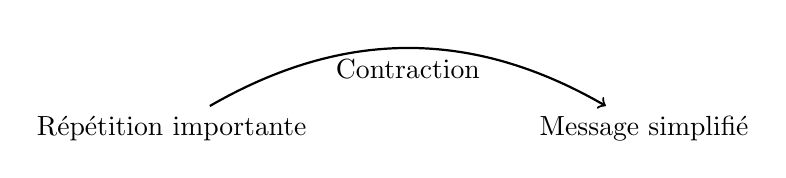
\begin{tikzpicture}
			\node (R) at(0,0) {Répétition importante};
			\node (M) at(6,0) {Message simplifié};
			\draw[->, thick] (R) to[bend left] (M);
			\node at(3,.75) {Contraction};
		\end{tikzpicture}
	\end{alertblock}
	\begin{exampleblock}{Exemples}
		\begin{itemize}
			\item Métro (\emph{Métropolitain}),
			\item Périph (\emph{Boulevard Périphérique}),
			\item Labo (\emph{Laboratoire}),
			\item ZZ...
		\end{itemize}
	\end{exampleblock}
\end{frame}

\begin{frame}
	\frametitle{Coût}
	\begin{alertblock}{Risques}
		\centering
		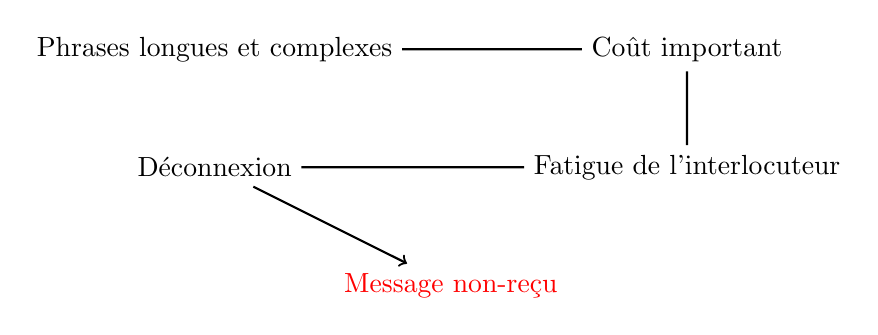
\begin{tikzpicture}
			\node (P) at (0,1.5) {Phrases longues et complexes};
			\node (C) at (6,1.5) {Coût important};
			\node (F) at (6,0) {Fatigue de l'interlocuteur};
			\node (D) at (0,0) {Déconnexion};
			\node[color=red] (R) at (3,-1.5) {Message non-reçu};
			\draw[->, thick] (P)--(C) (C)--(F) (F)--(D) (D)--(R);
		\end{tikzpicture}
	\end{alertblock}
	\begin{exampleblock}{Conséquence}
		\[ \text{Diminuer le nombre de signes} \implies \text{Message plus compréhensible} \]
		$\implies$ Phrases simples
	\end{exampleblock}
\end{frame} 
